\section{Introduction}

Simulation is often used to inspect various characteristics of a system.
In the SoOS project\footnote{See \url{http://www.soos-project.eu/} and \cite{soos} for details.} we inspect service-oriented aspects of operating systems.
One part of the project requires to simulate the interactions between software components of an operating system (in the following: OS) and between
OS and application software.

The key point is: it is not desirable to keep the whole, monolithic, OS kernel on each core of a multicore machine.
Doing so has detrimental effects on the caches of the individual cores \olcomment{find a better reference!}.
Moving to larger distributed systems, monolithic kernels hinder scalability as the entire internal state has to be synchronised amongst the copies.\jlcomment{Restate the paragraph after finding the reference!}
% \cbcomment{I don't think we should say more about S(o)OS or its ideas / concepts in the intro.}
% For example, we could dedicate some cores to an application and some cores to an OS.
% One possible approach to this is the partitioning of the address space. \olcomment{is this so?}
% In a simular manner, if we know that a core is occupied by a particular program, we can move the dynamic libraries, required for some other application to some other core's memory range.
% A further issue is the scalability of the parallel system.

Overcoming the aforementioned limitations of contemporary operating system designs is the motivation for the S(o)OS project \cite{soos}.
The project aims to research OS concepts and specific OS modules, which aid in scalability of the complete software stack (both OS and application) on future many-core systems.
One of the key concepts of S(o)OS is that only those OS modules needed by a application thread, are actually loaded into the (local) memory of a CPU core on which the thread will run.
This execution environment thus differs from contemporary operating systems where every core runs a complete copy of the (monolithic) operating system.

While creating new operating system concepts and regarding their interaction with the programmability of large-scale systems, we found that existing simulation packages do not seem to have the right abstractions for fast design exploration \cite{cotson,omnet}.
The ability to simulate separate components of the OS and of the application was the main goal to develop the OS simulator \soosim \cite{Baaij:2012}.
The design decisions were:
\begin{itemize}
\item To simulate message passing and shared memories as the main forms of communication between software components.
\item To have global \emph{ticks}, designating an abstract notion of progress.
\item To observe the number of ticks a component is: active, waiting for a response after invoking another component, or idle.
\end{itemize}
However, we additionally required a way to implement \emph{blocking} messaging as a means to provide \emph{synchronisation} between components.
In other words, if a blocking message is sent, the sender is waiting for the answer---regardless \emph{where} in the code of the sender the blocking \hs{invoke} method is called.
% If a blocking message is received, the reviever should suspend its current work and process the message.\olcomment{is this true?}
This means we required the notion of suspending a computation---it should be \emph{suspendable} at any moment of execution of the simulated component.
In the following we will show that using Haskell\nolinebreak[3] \cite{haskell-report} enabled us to implement this property in a nice way.
The contributions of this paper include:
\begin{itemize}
\item A short overview of the \soosim project.
\item The description of the embedded domain-specific language (eDSL) used to implement OS components in \soosim.
\olcomment{Do \hs{createComponent} etc. really form a DSL? Say `interface'?}
\item The description of \emph{a} eDSL to describe applications that will run on a \soosim \emph{simulated} system.
\item The list of Haskell language features, we found particularly useful in this project.
% \item \olcomment{in case of success: The way to model "suspending
%     computation" with heterogeneous data without using dynamic types.}
\end{itemize}
\soosim is also available from Hackage.\footnote{Issue \textsf{cabal install SoOSiM} to install \soosim. See also:
\url{http://github.com/christiaanb/SoOSiM}.}

The remaining part of this paper is organised as follows.
% Section~\ref{sec:soos-project} gives an overview of the SoOS project and of the role \soosim plays in the project.
Section~\ref{sec:soosim-an-overview} described the structure of the \soosim simulator from the user's perspective.
Section~\ref{sec:dsl} gives an implementation overview of the domain specific language, used to implement application running within a \soosim simulated environment.
Section~\ref{sec:impl-detail} discusses Haskell features from which our implementation especially benefited.
Section~\ref{sec:related-work} covers related work.
Section~\ref{sec:concl-future-work} concludes and gives an outlook for the further research.

% \section{SoOS Project}
% \label{sec:soos-project}
%
% The SoOS project \olcomment{....... } \cite{soos}...
% \olcomment{Do we need an overview of the whole project then?}\cbcomment{I don't think so} %% ok

\section{\soosim: An Overview}
\label{sec:soosim-an-overview}

\paragraph{Basic structure.}
The purpose of \soosim is to provide a platform that allows a developer to observe the interactions between OS modules and application threads.
For this reason the simulated hardware is highly abstract.

In \soosim, the hardware platform is described as a set of nodes.
Each \emph{node} represents a physical computing object: such as a core, complete CPU, memory controller, etc.
Every node has a local memory of potentially infinite size.
The layout and connectivity properties of the nodes are not part of the system description.
If such a level of detail is required, it would have to be modelled explicitly by the user.
\jlcomment{How?}
\olcomment{Is it possible to model these within \soosim, using various DSL implementations? If yes, say "In our design, embedded DSLs facilitate such definitions. See Section ... for details."}
\cbcomment{By creating a component, which would reside on each node, that handles the messaging.
Meaning that if you want to communicate with a component, you would invoke the messenger component, instead of the component itself.
The messenger module would then keep an internal state, representing the connectivity of all the nodes, and forward the message accordingly.}

Each \emph{node} hosts a set of components.
A \emph{component} represents an executable object: such as a thread, application, OS module, etc.
Components communicate with each other either using direct messaging, or through the local memory of a node.
Having both explicit messaging and shared memories, \soosim supports the two well known methods of communication.
Because multiple components can send messages to one component, all components have a message queue.
All components in a simulated system, even those hosted within the same node, are executed concurrently from the component's point of view.
The simulator poses no restrictions as to which components can communicate with each other, nor to which node's local memory they can read from and write to.
A user of \soosim would have to model those restrictions explicitly if required.
A schematic overview of an example system can be seen in Figure~\ref{fig:system}.

%\def\svgwidth{\columnwidth}
\begin{figure}
\centering
%\includesvg{system}
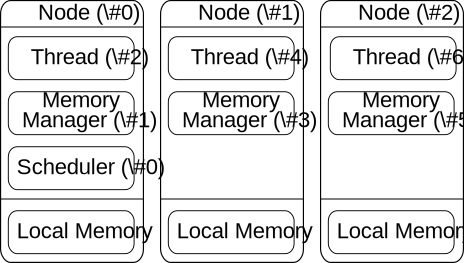
\includegraphics[width=0.7\linewidth]{system}
\caption{System, abstracted.}
\label{fig:system}
\end{figure}

\paragraph{Agility.}
Basic requirements that we would have towards any simulator include the facilities to straightforwardly simulate the instantiation of application threads and OS modules.
Aside from the fact that the S(o)OS-envisioned system will be dynamic as a result of loading OS modules on-the-fly, large-scale systems also tend to be dynamic in the sense that computing nodes can disappear (failure), or
appear (hot-swap).
Hence, we also require that our simulator facilitates the straightforward creation and destruction of computing elements, represented by \emph{nodes} in \soosim.
Our current need for a simulator rests mostly in formalising the S(o)OS concept, and examining the interaction between our envisioned OS modules and the application threads.
As such, being able to extract highly accurate performance figures from a simulated system is not a key requirement.
We do, however, wish to be able to observe all interactions among application threads and OS modules.
Additionally, we wish to be able to \emph{zoom in} on particular aspects of the behaviour of an application: such as memory access, messaging, etc.

The simulator \emph{attempts} to progress all components concurrently in one discrete step called a \emph{tick}.
If a component is waiting for a response from an invoked component, but none is available, a component will remain in a waiting state.
During a tick, the simulator progresses a component by one of the following means:
\begin{itemize}
  \item If a component is in a waiting state, and a response is available in the message queue, the component will be executed with this response message.
  \item If a component is not in a waiting state, and the message queue is not empty, the component will be executed by passing it the message that is at the head of the message queue.
  \item If a component is not in a waiting state, and the message queue is empty, the component will be executed by passing it a \emph{null} message.
\end{itemize}
When desired, a component can inform the simulator that it does not want to receive these null messages.
In that case the component will not be executed by the simulator during a \emph{tick}.

The simulator keeps several statistics with regards to the components, including how many ticks a component was either: \emph{active}, \emph{waiting}, or \emph{idle}.
When a component makes progress during a tick, is considered \emph{active}.
When a component does not make progress because the response it was waiting for was not yet available, the component is designated as \emph{waiting}.
A component not making progress because it has an empty message queue, and having indicated that it does not want to receive \emph{null} messages, is designated as \emph{idle}.

\subsection{OS Component Descriptions}
The OS components are also specified in Haskell, each component is modelled as a function.
In case of \soosim, such a function is executed within the context of the simulator, this means: in a \emph{monad}.

Because the function is executed within the monad, it can have \emph{side-effects} such as sending messages to other components, or reading the local memory of a node.
In addition, the function can be temporarily suspended at (almost) any point in the code.
\soosim needs to be able to suspend the execution of a function so that it may emulate synchronous message passing between components, a subject we will further elaborate later on.

We describe a component as a function that receives a user-defined internal state as its first argument, and a value of type \hs{SimEvent} as its second argument.
The result of this function is the internal state.
A value of type \hs{SimEvent} is either message from another component, or a null message.
We thus have the following \emph{general} type signature for a component:
%\numbersoff
\begin{code}
component :: state -> SimEvent -> SimM state
\end{code}

The simulator monad \hs{SimM} is described in Figure~\ref{fig:code-simm} in Section~\ref{sec:impl-monads}.
The user-defined internal \hs{state} can be used to store any information that needs to perpetuate across simulator ticks.
\hs{state} should be read as a placeholder for any (user-defined) datatype; there is no actual predefined \hs{state} datatype.

To include a component description in the simulator, the developer will have to create an instance of the \hs{ComponentIface} \emph{type class}.
% A \emph{type class} in Haskell can be compared to an interface
% definition as those known in object-oriented languages.  An
% \emph{instance} of a \emph{type class} is a concrete instantiation
% of such an interface.
%% haskell people know that!
The \hs{ComponentIface} requires the instantiation of the following values to completely define a component:

\begin{itemize}
  \item The initial internal state of the component.
  \item The unique name of the component.
  \item The monadic function describing the behaviour of the component.
\end{itemize}

Note, we are aiming at a high level of abstraction for the behavioural descriptions of our OS modules, where the focus is mainly on the interaction with other OS modules and application threads.


\subsection{Interaction with the Simulator}

%% we agreed on not having this figure
% \begin{figure*}
% \centering
% \begin{code}
% createComponent :: Maybe NodeId -> Maybe ComponentId -> String -> SimM ComponentId   -- Nothing is self
%
% -- Synchronously invokes another component
% invoke :: Maybe ComponentId -> ComponentId -> Dynamic -> SimM Dynamic  -- the invocation argument has to be like this
%
% ...
% \end{code}
% \caption{The interaction interface.}
% \label{fig:comp-types}
% \end{figure*}

Components have several functions at their disposal to interact with the simulator and consequently interact with other components.
% We show the types of these functions in Figure~\ref{fig:comp-types}.
The available functions are:

\paragraph{\hs{createComponent}}
instantiates a new component on a specified node.
\paragraph{\hs{invoke}}
sends a message to another component and wait for the answer.
Whenever a component uses this function it will be temporarily suspended by the simulator.
Several simulator ticks might pass before the response.
Once the response is available the simulator resumes the execution of the calling component.
\paragraph{\hs{invokeAsync}}
sends a message to another component and register a handler with the simulator to process the response.
In a contrast to \hs{invoke}, using this function will \emph{not} suspend the execution of the component.
\paragraph{\hs{respond}}
sends a message to another component as a response to an invocation.
\paragraph{\hs{yield}}
informs the simulator that the component does not want to receive null messages.
\paragraph{\hs{readMem}}
performs a read at a specified address of a node's local memory.
\paragraph{\hs{writeMem}}
writes a new value at a specified address of a node's local memory.
\paragraph{\hs{componentLookup}.}
This function performs a lookup of the unique identifier of a component on a specified node.
Components have two unique identifiers, their global \emph{name} (as specified in the \hs{ComponentIface} instance), and a \hs{ComponentId} that is a unique number corresponding to a specific instance of a component.
When a programmer wants to \emph{invoke} a component, she needs to know the unique \mbox{\hs{ComponentId}} of the specific instance.
To give a concrete example, using the system from Figure~\ref{fig:system} as our context: \emph{Thread (\#6)} wants to invoke the instance of the \emph{Memory Manager} that is running on the same Node (\#2).
As \emph{Thread (\#6)} was not involved with the instantiation of that OS module, it has no idea what the specific \hs{ComponentId} of the memory manager on Node \#2 is.
It knows the unique global name of all memory managers, so it can use the \hs{componentLookup} function to find the \hs{Memory Manager} with ID \#5 that is running on Node \#2.

\subsection{Synchronisation between Modules}
% \olcomment{is it clear, that FSM is standard approach, not coroutines?}\cbcomment{I hope the following subsection explains our use of coroutines better} %% yes
A \emph{naive} approach to model synchronisation between OS modules is to implement an OS module as a finite state machine (FSM).
In state `X' OS module `Bob' could send a message to `Alice' and enter state `Y'.
Only when receiving a response from `Alice', would `Bob' progress from state `Y' to state `Z'.
If we wanted, we could even implement OS modules as \emph{pure} functions, which, aside from returning an updated state, would also return a simulator event.
One such event would then be sending a message to another component.

When sending a message the FSM would enter a new state for that specific invocation of another component.
As a result, designers of OS module descriptions would have to extend the dictionary of states for \emph{every} invocation their module makes.
As one can imagine, the explicit FSM approach quickly resulted in overly verbose and unstructured OS module descriptions.

As a solution we essentially mechanised the creation of the FSM using the notion of \emph{suspendable} computations.
When a developer uses the \hs{invoke} function, two things actually happen:
\begin{itemize}
  \item A message is send to the invoked component (callee).
  \item The remaining computation of the caller is suspended and stored by simulator, ready to be scheduled once a response to the invocation arrives.
\end{itemize}
Every call to \hs{invoke} hence corresponds to an explicit state transition, but without the burden of explicit state-keeping.
We achieved suspendability using coroutines~\cite{coroutines}, more specifically, a coroutine monad transformer~\cite{cmt}.
We return to the subject of the coroutine monad transformer in Section~\ref{sec:impl-detail}.

\section{A Domain-Specific Language for \soosim}
\label{sec:dsl}
One of the purposes of \soosim is to observe the interaction between application and OS.
We however do not want to \emph{pollute} our application descriptions with calls to the simulator functions.
Nor do we want to be forced to describe our application in a monadic style.
Additionally, we want to be in control which interactions between OS and application are exactly simulated, without having to change either the descriptions of the OS modules or the application when we want to observe different aspects.

For the above reasons we have chosen to make use of embedded languages for the definitions of our applications.
The idea is to specify an application once in a self-created embedded language and define different interpretations for the embedded language constructs as the observations of the interaction between application and OS\nolinebreak[3]  \cite{Hofer:2008:PED:1449913.1449935}.
% \olcomment{the cited paper is about different interpretations of the same code!}

Following the \emph{final tagless} \cite{final_tagless_embedding} encoding of embedded languages in Haskell, we use a type class to define the language constructs.
As an example we demonstrate a mini functional language with mutable references.\olcomment{was: "running example".}
A partial specification of the \hs{Symantics} (a pun on \emph{syntax} and \emph{semantics} \cite{final_tagless_embedding}) type class, defining an \emph{embedded language}, is shown in Figure~\ref{fig:embedded_language_interface}.
The arrow \hs{:->} is the function arrow in the embedded language, \eg \hs{repr (a :-> b)}, in contrast to the function arrow \hs{->} of the host language.

\begin{figure}
%\centering
\begin{code}
class Symantics repr where
  lam   :: (repr a -> repr b) -> repr (a :-> b)
  app   :: repr (a :-> b) -> repr a -> repr b

  drf   :: repr (Ref a) -> repr a
  (=:)  :: repr (Ref a) -> repr a -> repr Void
\end{code}
\caption{An embedded language, a fragment. Viz.~\cite{final_tagless_embedding}}
\label{fig:embedded_language_interface}
\end{figure}

One interaction we might now want to observe is the application's use of mutable references and the subsequent communication with the memory manager OS module.
For this purpose we create a \hs{newtype RefMemAcc} wrapping the simulator monad, and define an instance of the \hs{Symantics} type-class for it.

We can define most language constructs to behave like their Haskell counterpart, e.g., the \hs{app} construct instance is defined using monadic bind (\hs{>>=}\xspace).
%($\mathit{>>=}$).
However, instead of using a Haskell-based implementation like \textsf{Data.IORef} for the definition of the mutable reference aspect of our language, we implement these constructs as invocations of the memory manager (see Figure~\ref{lst_observing_memory_access}).

\begin{figure}
%\centering
\begin{code}
newtype RefMemAcc =  RMA SimM

instance Symantics RefMemAcc where

  drf x = RMA $ do
    i     <-- foo x
    mmId  <-- componentLookup "MemoryManager"
    fmap unmashal $ invoke mmId (marshal (Read i))

  x =: y = RMA $ do
    i     <-- foo x
    v     <-- bar y
    mmId  <-- componentLookup "MemoryManager"
    fmap unmashal $ invoke mmId (mashal (Write i v))
\end{code}
\caption{Observing memory access (partial definition).}
\label{lst_observing_memory_access}
\end{figure}


% \begin{figure}
% \centering
% \begin{code}
% data SchedulerState = ... -- basically obtains two lists
%
% scheduler :: a -> ComponentInput -> SimM a
% scheduler = ... -- implementation omitted
%
% instance ComponentIface  SchedulerState where
%   initState           =  SchedulerState [] []
%   componentName _     =  "Scheduler"
%   componentBehaviour  =  scheduler
% \end{code}
% % createComponentRequest :: String -> SimM ComponentId
% % createComponentRequest =  ... -- implementation omitted
% \caption{Registering a \hs{scheduler} component.}
% \label{fig:code-scheduler}
% \olcomment{so what?}
% \end{figure}

% \subsection{Final Tagless}
%
% \olcomment{- Final tagless \cite{final_tagless_embedding}
%
% - Tillmann embedded DSL with type classes
% \cite{Hofer:2008:PED:1449913.1449935}
%
% - I am refreshing this paper ATM.
%
% - 2006: typed interpreter of a typed language cannot be tagless. final tagless paper says: wrong!
% }

\paragraph{Final tagless embedding.}
\citeauthor{final_tagless_embedding} have demonstrated how a typed interpreter of a typed language can be tagless \cite{final_tagless_embedding}.
This approach does not use GADTs or dependent types.
The target language types are represented as host language types, object terms are encoded as calls to host language functions. With type classes \citeauthor{final_tagless_embedding} make it possible to express, \eg an interpreter and an compiler of the same language in a flexible manner.
\citeauthor{Hofer:2008:PED:1449913.1449935} do a similar work \cite{Hofer:2008:PED:1449913.1449935}, but focus on different interpretations.
This matches our intentions.
We use our above example of a small language with mutable references.
If we want to observe memory interactions in a more detail, we embrace an additional implementation of the language, where the functions for the memory interaction are exactly studied and basically ignore the observation of other parts of the language.
In a similar manner we can introduce further implementation of the same language with different properties.

\section{Features We Used}
\label{sec:impl-detail}

\subsection{Existential Types}
We employ existential type to store the differently typed states of all the components running in our simulated environment.
Components are subsequently implemented as type class instances, giving us a straightforward way to access the existentially quantified values in our collection of states.

\subsection{Type classes}
Type classes are naturally used for the eDSL encoding from the previous section \cite{Hall:1996:TCH:227699.227700,final_tagless_embedding}.

Beyond this, we use type classes to express many other useful abstractions.
For instance, an \emph{interface} for the component of the OS is a type class.
Thus, each interacting `building block' in the simulated software is an instance of that particular type class.
Although initially used solely for the purpose of dealing with existentially quantified values, this \hs{ComponentIface} type class enables great flexibility, including an option to extend the kinds of simulated objects by third party.

\subsection{Monads}
\label{sec:impl-monads}
\begin{figure}
%\centering
\begin{code}
type SimMonad  =  StateT SimState IO
data SimState  = ...

newtype SimM a
  = SimM { runSimM ::
               Coroutine
                 (RequestOrYield CompID Dynamic)
                 SimMonad
                 a
         }
    deriving (Functor, Monad)

data RequestOrYield request response x
  =  Request request (response -> x)
  |  Yield   x

instance Functor (RequestOrYield x f) where
  fmap f (Request x g)  = Request x (f . g)
  fmap f (Yield y)      = Yield (f y)
\end{code}
\caption{Implementing \hs{SimM}.}
\label{fig:code-simm}
\end{figure}

We use a monad called \hs{SimM} to capture the \emph{state} of the simulator.
The implementation of \hs{SimM}, sketched in Figure~\ref{fig:code-simm}, enables us to reach the main implementation goal: the ultimate suspension and resumption of the components upon message passing.
To suspend a computation in the current component we can now merely write \hs{request componentId}, where the \hs{componentId} is the unique ID of some other component.
The suspending of a component is nothing else than sending a outgoing message in the name of the component and blocking the sender until a response.
The execute a resumeable computation we issue \hs{resume} \mbox{\hs{computation}.} %% hackery to get spaces right


\subsection{Coroutines}
\label{sec:impl-coroutines}
As we mentioned above and as one could infer from Figure~\ref{fig:code-simm}, the implementation makes use of the coroutines~\cite{coroutines}.
With this concept we capture the notion of multiple suspending and resuming computations.
The need in such a behaviour arises naturally with the blocking message passing between components.
We utilise \textsf{Control.Monad.Coroutine} \cite{cmt} to express coroutines.

\subsection{Dynamic Types}
We use dynamic types \cite{Abadi:1991:DTS:103135.103138} as `the other side' of the type classes: we need to communicate heterogeneous types over a typed channel, and there is no option to know all the types-to-transmit at the moment of the channel definition.

The \emph{origin} for the need of dynamic types lies in the suspension functor or our coroutines.
More specifically, the \hs{response} field, that designates the type of the response returned after an invocation.
This field would be different for every component we want to invoke, as components should be able to communicate datatypes of any kind.
We have only been able to encode this aspect in the suspension functor using dynamic types.

% \cbcomment{The use-case for existentials+type-classes is to get an OO-like way of programming; please correct me if I'm wrong.
% Just take a look at: http://www.haskell.org/haskellwiki/Existential_type
% This approach is perfect if you know upfront what kind of operations you want to perform on the data-types.
% The wiki demonstrates this with an example of a type-class that determines the perimeter and area of different datatypes representing geometric shapes.
% And indeed, you can put different shapes in a homogeneous collection, and calculate the area and perimeter for the different types of shapes in this collection.

% The use case in SoOSiM is however far different: we do NOT know, upfront, how the data-types will be used.
% The information stored in these values can and should be be manipulated in any kind of way.
% Trying to define a type-class 'Foo' would either be too large, or too restrictive.

% So I really think that 'Dynamic' is the 'answer' to our problem, although it is an ugly one.}

If we knew upfront what kind of operations the users might want to perform on the data types, we could have used existential types and type classes, \viz \cite{Laufer:1994:PTI:186025.186031,Kiselyov:2004:STH:1017472.1017488}.
However, this is not our case.
\olcomment{I connect the dynamic types to communication, as we need the coroutines for blocking!}
We need to transmit synchronously values of heterogeneous types.
% and the information on how these values should be used is stored in the values themselves!
% This information should be be manipulated in any kind of way.
The types in the coroutine monad transformer are too restrictive.
Trying to define a type class or a sum type for this setting would yield either a too large, or a too restrictive definition.
%We are not aware of any other way to implement this behaviour.
%
We utilised \textsf{Data.Dynamic} to convert transmitted values of a dynamic type into values of concrete monomorphic types.
% \olcomment{only if it works out:}
% However, recently we have found a better solution that allows us to refrain from dynamic type. We discuss it below.
% \olcomment{here goes the real reason, check if all above still applies}
An attempt to sort the dynamic types out with the parameterised monad also fails, as detailed in the next section.

\subsection{Parameterised Monads}
The parameterised monads\footnote{See \url{http://www.haskell.org/pipermail/haskell-prime/2006-February/000498.html}.}  allow more generic type signatures for monad operations, esp.\ for \hs{>>=}\xspace\nolinebreak[4] \cite{monad-parametrisable}:
\begin{code}
class PMonad m where
return :: a -> m s s a
(>>=)  :: m s1 s2 a -> (a -> m s2 s3 b) -> m s1 s3 b
\end{code}
If we could change the from one to another intermediate type in the coroutine, we would need no dynamic types.
This approach works fine with the state monad
\begin{code}
newtype PState s1 s2 a
  = PState { runPState :: s1 -> (a, s2) }

instance PMonad PState where
return a = PState $ \s -> (a, s)
m >>= k  = PState $ \s -> let (a, s') = runState m s
                         in runState (k a) s'
\end{code}
but it fails for the coroutines.
The pivotal issue is: if we introduce different types for the intermediate states of the coroutine, we end up adding more and more types --- the coroutine definition is recursive.
In this (non proper Haskell) code
\begin{code}
newtype Coroutine m o i r
  = Coroutine { resume :: m (Either (o, i
     -> Coroutine m i2 o r)  r) }
\end{code}
we make an attempt to reach our goal.
Let us abbreviate left and right hand side of the above equation with LHS and RHS.
However, to make this code valid Haskell, we need to reference \hs{i2} on the LHS: \hs{Coroutine m i i2 o r}.
In the type of the \hs{resume} function on the RHS we need to reference \hs{Coroutine} correctly, hence we write \hs{Coroutine m i2 i3 o r} there. 
We need to add \hs{i3} on the LHS, and so on.
Using some more advanced tricks, like a type class for all the chain \hs{i}, \hs{i2}, \hs{i3}, \dots\ does not really help: all the types on the RHS still need to be listed on the LHS, thus exploding the definition.

%% this is for the case it works. It does not.
% \paragraph{What we did.} We implemented the coroutine monad transformer for the parameterised monads \olcomment{show some code?}.
%
% \paragraph{What we miss.} Since GHC seems to assume that each bind has the type \hs{Monad m => m a -> (a -> m b) -> m b} when desugaring the \hs{do}-notation, we were forced to use explicit \hs{>>=}\xspace instead.

\section{Related Work}
\label{sec:related-work}

\paragraph{Operating systems and simulators.}
COTSon \cite{cotson} is a full system simulator that allows a developer to execute normal x86 code in a simulated environment.
COTSon is far too detailed for our needs, and does not facilitate the easy exploration of a complete operating system.

OMNeT++ \cite{omnet} is a C++-based discrete event simulator with focus on parallel systems. OMNeT++ is too static for our purposes, it disallows dynamic modules.


\citeauthor{house} describe a basic operating system implementation in Haskell called House \cite{house}.
This work is in a sense dual to ours: we simulate an OS.
\citeauthor{house} modified GHC run-time system to allow code execution on bare metal.
In House, OS modules are executed within the \hs{Hardware} monad, allowing direct interaction with real hardware.
This approach is comparable with our \hs{SimM} monad.
However, as we are more concerned with interaction of OS modules, House in not suitable for our purposes:  OS modules in House must be implemented in full detail.

Barrelfish \cite{barrelfish} is an OS in which domain-specific languages are used, amongst other purposes, to define driver interfaces.
These embedded languages are also implemented in Haskell.
The approach used in Barrelfish is however to create parsers for their languages, in a contrast to our embedding approach.


\paragraph{Embedded domain-specific languages.}
Embedding programming languages was proposed by \citeauthor{Landin:1966:NPL:365230.365257} \cite{Landin:1966:NPL:365230.365257}.
For the concept of an eDSL see the papers by \citeauthor{hudak1} \cite{hudak1,hudak2}, the 1998 paper describes pure embedding.
The literature on this topic is quite broad, an overview is presented, \eg by \citeauthor{dsl-survey} \cite{dsl-survey}.

The final tagless embedding of DSLs originates from the seminal paper by \citeauthor{final_tagless_embedding} \cite{final_tagless_embedding}.
\citeauthor{Hofer:2008:PED:1449913.1449935} \cite{Hofer:2008:PED:1449913.1449935} presented a paper that compared to the work by \citeauthor{final_tagless_embedding} \cite{final_tagless_embedding} is more composable, allows subtyping, and is done in Scala \cite{odersky2008programming}.
These two papers have different goals: \citeauthor{final_tagless_embedding} implement DSLs for higher-order languages, while \citeauthor{Hofer:2008:PED:1449913.1449935} focus on the possibility to plug in multiple interpretations of a pure embedded DSL.
The latter corresponds more with our goals: we want control over what we observe in the particular instance.

\paragraph{Suspendable computation.} We used coroutines monad transformer \cite{cmt} to express a suspendable computation.
Other approaches to this include the suspension monad implementations of iteratees/enumeratees. This approach was introduced in \cite{oleg-iteratee}, see, \eg an overview by \citeauthor{lato2010iteratee} \cite{lato2010iteratee}.
See also Oleg Kiselyov's new paper \cite{springerlink:10.1007/978-3-642-29822-6_15} for the current description of iteratee-based IO in Haskell.

\paragraph{Haskell experience reports.}
Haskell has been successfully used to implement a range of applications far from typical programming language research.
This is not surprising for a general purpose language, but nevertheless we would like to list most interesting applications.
We already mentioned House \cite{house} in the previous section.

Haskell has been used to facilitate a formal verification of a
microkernel \cite{Klein:2009:ERS:1631687.1596566}, to implement
commercial mission-critical applications
\cite{Sampson:2009:ERH:1631687.1596578}, to manage a Linux
distribution \cite{Beshers:2007:ERU:1291220.1291184}, to configure
realtime OS components \cite{Jones:2008:ERP:1411203.1411219}, etc.

\section{Conclusions and Future Work}
\label{sec:concl-future-work}

\paragraph{Conclusions.}
We have presented the efforts required to implement \soosim, an OS simulator in Haskell.
We note that the techniques more commonly used in the programming language research were highly applicable for our purposes.

We have demonstrated how the utilisation of final tagless eDSL construction \cite{final_tagless_embedding,Hofer:2008:PED:1449913.1449935}, type classes \cite{Hall:1996:TCH:227699.227700}, monads \cite{Wadler:1990:CM:91556.91592}, \hs{Dynamic} types \cite{Abadi:1991:DTS:103135.103138}, and coroutines \cite{coroutines,cmt} facilitated an abstract and concise implementation of an operating system simulator.
% \olcomment{in case of success: We found a way to replace \hs{Dynamic} types with parameterised monads \cite{monad-parametrisable} in our setting.}
% \olcomment{These techniques belong to the typical repertoire of a programming language designer, but not of an operating systems researcher. --- emphasise somehow, that it is uncommon to use all these for such a task, which makes our work stand out , this this work is cool.}
It is uncommon to use all these features for such a task --- a fact that emphasises the novelty of our work.

\paragraph{Real life simulations.}
The major goal of the project is to simulate the behaviour of a real life application and to draw conclusions therefrom.
%This work is still ongoing.
We are currently actively researching these issues.

\paragraph{Concurrency.}
One aspect of the future work is the concurrent \soosim.
One option is to use Concurrent Haskell \cite{ConcHs}, it provides (concurrent) green threads.
However, it would also require to use software transactional memory \cite{springerlink:10.1007/s004460050028} because of multiple writes to the same data.
Examples of fruitful combinations with other concepts include papers by \citeauthor{Harris:2008:CMT:1378704.1378725} \cite{Harris:2008:CMT:1378704.1378725} and \citeauthor{Bieniusa:2010:BAA:1835698.1835714} \cite{Bieniusa:2010:BAA:1835698.1835714,springerlink:10.1007/978-3-642-25959-3_2}.
Another option would be to use a \emph{parallel} Haskell like Multicore Haskell \cite{marlow:rsm}, \hs{Par} monad \cite{par-monad} or Eden \cite{eden}.
The `multiple writes' issue, however, needs some further handling in this case.
Two further options are either to make the coroutine execution concurrent using actors~\cite{Hewitt:1973:UMA:1624775.1624804,sulzmann2008actors} or to switch to iteratees for expressing blocking communication and to utilise transformers from usual to parallel composable iteratees\footnote{See \url{http://projects.haskell.org/pipermail/iteratee/2011-July/000083.html} for details.}.

% \appendix
% \section{Appendix Title}
%
% This is the text of the appendix, if you need one.

\acks

%Acknowledgments, if needed.
This work was supported by the S(o)OS project, sponsored by the European Commission under FP7-ICT-2009.8.1, Grant Agreement No.~248465.
We thank Chung-chieh Shan and Oleg Kiselyov for valuable remarks on
\hs{Dynamic} types and the parallel iteratees correspondingly.

%%% Local Variables:
%%% mode: latex
%%% TeX-master: "soosim"
%%% End:
